%\documentclass{beamer}
%\usetheme{Pittsburgh}
\documentclass{scrartcl}

\usepackage[utf8]{inputenc}
\usepackage{default}
\usepackage[procnames]{listings}
\usepackage{graphicx}
%\usepackage[toc,page]{appendix}
\usepackage{caption}
\usepackage{hyperref}
\usepackage{color}
%\usepackage{csvsimple}
\usepackage{float}
%\usepackage[T1]{fontenc}



%Bibliogrpahy?
%\usepackage{bibentry}
%\nobibliography*
%\bibentry{ }


%Python
\definecolor{keywords}{RGB}{255,0,90}
\definecolor{comments}{RGB}{0,0,113}
\definecolor{red}{RGB}{160,0,0}
\definecolor{green}{RGB}{0,150,0}
\lstset{language=Python,
    basicstyle=\ttfamily\scriptsize,
    keywordstyle=\color{keywords},
    commentstyle=\color{comments},
    stringstyle=\color{red},
    identifierstyle=\color{green},
    breaklines = true,
    columns=fullflexible,
    %Numbering and tabs
    %numbers=left,
    %numberstyle=\tiny\color{gray},
    %stepnumber=2,
    %numbersep=1em,
    tabsize=4,
    showspaces=false,
    showstringspaces=false}

\begin{document}

\title{Learning and Adaptivity}
\subtitle{Report No. 3}
\author{
  \href{daiem.ali@smail.inf.h-brs.de}{Ali, Daiem}: \href{https://github.com/daiemna}{github.com/daiemna}\\
  \href{christophe.quignon@smail.inf.h-brs.de}{Quignon, Christophe}:\href{https://github.com/ChrisQuignon}{github.com/ChrisQuignon}
  %Familyname, Name
}
\date{\today}


\maketitle

%TODO: add abstract and conclusion
%labels (or zero)
%references (or zero)
%remove scaffolding code


\begin{abstract}
\textbf{Abstract:}
\end{abstract}

\section{Correlation}
\label{sec:correlation}
We rearranged the correlation to have a better visual overview of the linking of the features. We ordered the correlation to maximize the clusters of similar correlation. As seen in figure \ref{fig:correlation} we have at least three clusters of features with similar correlation:

\begin{enumerate}
\item Energy, power, volumetric flow rate
\item Outside temperature, input temperature, output temperature
\item Outside temperature, precipitation, relative air humidity
\end{enumerate}

Remarkably those three groups have a meaning in the system. The first group contains the features to control the system, the second group contains all features that describe the system and the third group is the input to the system, where the outside temperature clearly dominates the group.

\begin{figure}[H]
  \centering
  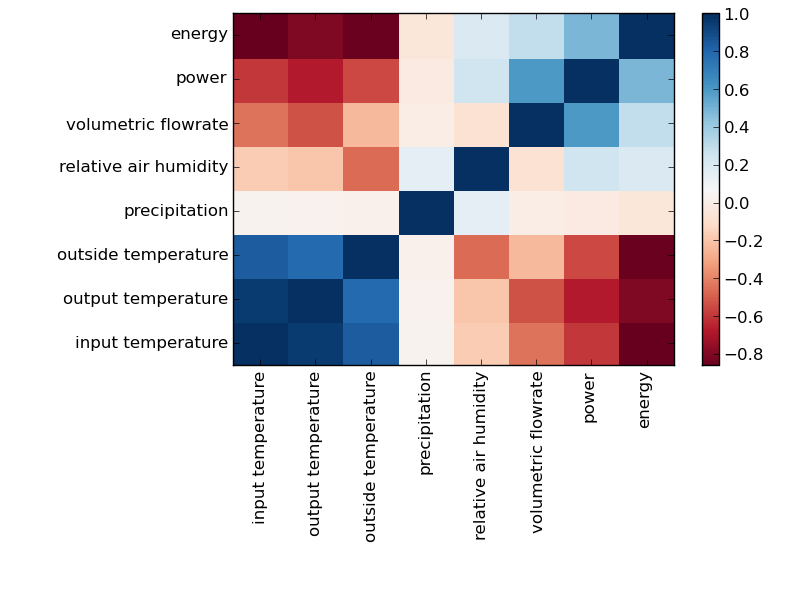
\includegraphics[width=0.5\linewidth]{img/correlation.png}
  \caption{Correlation matrix of all features.}
  \label{fig:correlation}
\end{figure}
%PUT UNITS ON THE FIGURES

\section{Sliding Window}
\label{sec:slidingwindow}
As suggested in \cite{vafaeipour2014application} the sliding window approach was used to learn how to predict. In this approach the time series is split into windows or frames of input and output. Unlike in regression learning, those windows are shifted. Thus the learning algorithm does not learn the relation of the features at the same time, but their relation in the future. With this approach, it is possible to include all features as an input and select few of them as an output. This can be enhanced further by including predictable features into the input. These three methods are depicted in Figure \ref{fig:slidingwindow}.\\
The random forest implementation we are using however can not handle input with more than one dimension. Thus we flatten the input to one dimension. Since the feature values are typically easily separable, we expect the random forest to recognize this flattening in an early step. We do not include this as an extra information into the trees.

\begin{figure}[H]
  \centering
    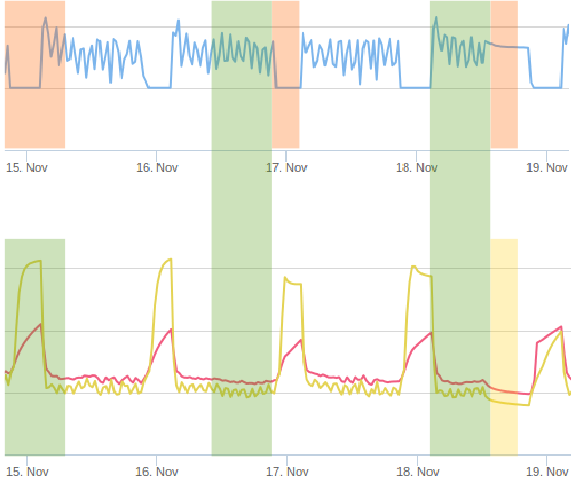
\includegraphics[width=0.5\linewidth]{img/regpred.png}
  \caption{Input(green) and output(red) frames for regression(left), prediction(middle) and enhanced prediction(right).}
  \label{fig:slidingwindow}
\end{figure}
%PUT UNITS ON THE FIGURES

\section{Seasonal decomposition}
\label{sec:season}
Much like spatial data, seasonal data can be decomposed as shown by \cite{loess}. Given the range of the season, one an identify an overall trend, a cyclic seasonal aspect and a residual which describes the system. As seen in figure \ref{fig:decomp} this decomposition helps to identify significant aspects of the time series. In figure \ref{fig:season} we see a zoom on the seasonal aspect. For one week, the repetitive pattern of one day is visible. The similarity is remarkable.


\begin{figure}[H]
  \centering
  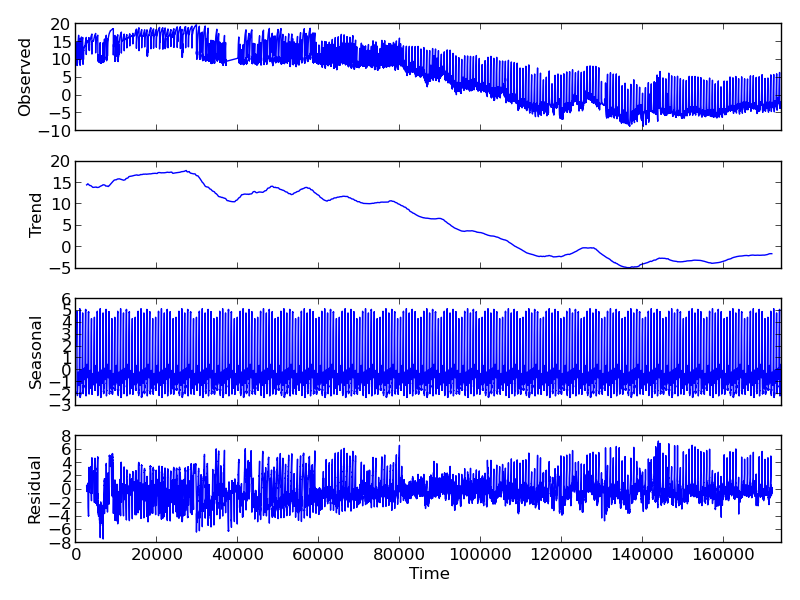
\includegraphics[width=0.5\linewidth]{img/seasondecomposition-input-temperature.png}
  \caption{Seasonal decomposition of the input temperature. Time in two minutes steps.}
  \label{fig:decomp}
\end{figure}
%PUT UNITS ON THE FIGURES

\begin{figure}[H]
  \centering
  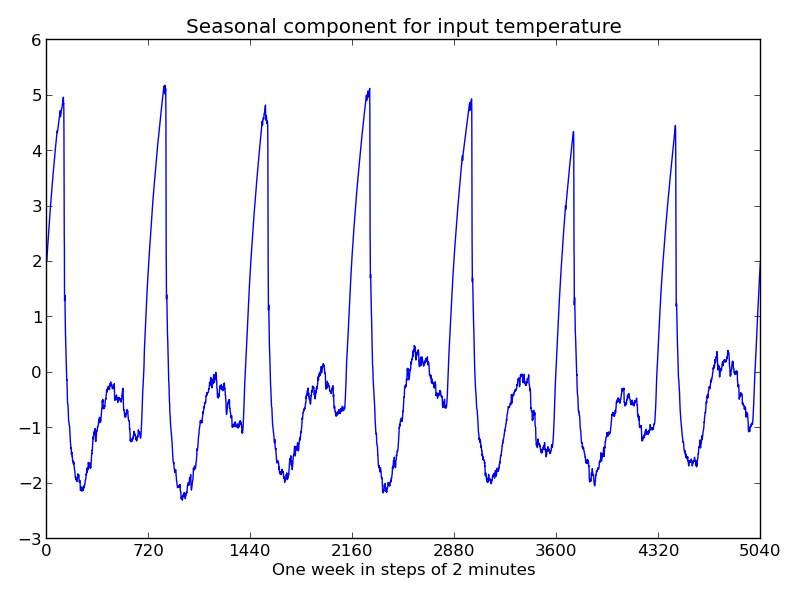
\includegraphics[width=0.5\linewidth]{img/season-input-temperature.png}
  \caption{One week season of the input temperature.}
  \label{fig:season}
\end{figure}
%PUT UNITS ON THE FIGURES


\section{Timeshift}
As explained in the section \ref{sec:slidingwindow} we have different frames for the input and the output. These frames however can have a sever impact for the learning. The position as well as the size has an impact on information included and thus can affect the learning. If a trend is not included in the frame it can not be learned. On the other hand, a large frame significantly increases learning time. We aim to have an input frame size that includes enough information for a trend and an output frame size that covers the results of the input. The amount of information within the frames can be scaled by subsampling.\\
The critical point here is the size of the output frame. Once we have a change in the input the output frame must cover the time where the changed input affects the output. To find this delays, we analysed the correlation of the seasonal part of the time series as explained in section \ref{sec:season}. Figure \ref{fig:timeshift} show the time shift for the maximum correlation between the features. One can see the same groups as in the regular correlation (See Section \ref{sec:correlation}). This means that the different sub parts of the system have different delays, varying between a few minutes and 4 hours.\\
Interpreting these shifts is not trivial, for features with a low correlation they may be discarded, because they probably do not cause each other but to a different input as the time of the day. For the small delay between the input and the output temperature the delay simply is the time the liquid travels. For the delay between the outside temperature and the energy this is probably the delay caused by the physics of the building.\\
However, 4 hours seems to be a reasonable frame size.


\begin{figure}[H]
  \centering
  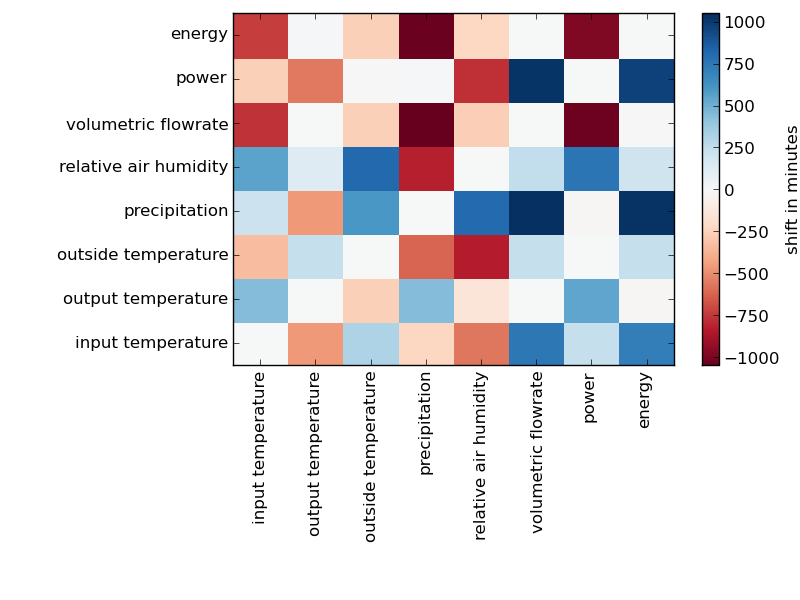
\includegraphics[width=0.5\linewidth]{img/timeshift.png}
  \caption{The timeshift in minutes for the optimal correlation between the seasonal timeseries.}
  \label{fig:timeshift}
\end{figure}
%PUT UNITS ON THE FIGURES

\section{Conclusion} 
%TODO



%BIBLIOGRPAHY?
\bibliographystyle{plain}%amsalpha
\bibliography{bib.bib}
%\bibentry{}

%\begin{appendix}
%\section{}

%\end{appendix}


%COPY AND PASTE FROM HERE

%\begin{enumerate}
% \item
%\end{enumerate}

%\href{link}{text}

%\begin[Language=Python]{lstlisting}
%#PYTHON CODE HERE
%\end{lstlisting}

%\lstinputlisting[language=Python]{	}

%\csvautotabular[separator=semicolon]{data.csv}


%\begin{figure}[H]
%  \centering
%  \includegraphics[width=0.5\linewidth]{../img/	}
%  %\caption{}
%  %\label{fig:}
%\end{figure}
%PUT UNITS ON THE FIGURES

\end{document}
